\documentclass{article}

\usepackage{homework}

\course{Encryption}
\assignment{Homework 1}

\begin{document}
\homeworktitle

\begin{enumerate}[label={}]
	\item \textbf{Task 1:} Affine cipher in $\Z_{97}$.
	\begin{enumerate}
		\item Encryption and Decryption functions with key $k=(a,b)$ (the message is $m$ and the resulting ciphertext is $c$):
		\begin{align*}
			E(k, m) &= a \cdot m + b \bmod 97\\
			D(k, c) &= a^{-1} \cdot (c - b) \bmod 97
		\end{align*}
		\item The number of possible meaningful and different keys is \[ \lvert a \rvert \cdot \lvert b \rvert \]
		Where $\lvert a \rvert$ is the possibilities for $a$ and $\lvert b \rvert$ is the different possibilities for $b$. $b$ can have 97 different values, and $a$ can have as many as there are co-primes below 97 with 97. This is given by Euler's Totient function: $\phi(97) = 96$ (this is because 97 is prime).\\
		In total the number of different keys is: 
		\[96 \cdot 97 = 9312\]
		\item We have an intercepted ciphertext-plaintext pair: (DOG)=(28 83 43), and a ciphertext with the same key: (78 23 33).\\
		To figure out the key we can use two letters from the known ciphertext-plaintext pair with either the Encryption or the Decription functions: (I choose the decryption with letters (DO) = (28 83))
		\begin{align*}
			D(k, 28) &= a^{-1} \cdot (28 - b) \bmod 97 = (D)3\\
			D(k, 83) &= a^{-1} \cdot (83 - b) \bmod 97 = (O)14
		\end{align*}
		Thus we get:
		\begin{align*}
				a^{-1} \cdot (28 - b) \bmod 97 &= 3\\
				a^{-1} \cdot (83 - b) \bmod 97 &= 14
		\end{align*}
		Rewriting the equations we get:
		\begin{align*}
			b &= 28 - 3a \bmod 97\\
			b &= 83 - 14a \bmod 97
		\end{align*}
		Making the two equal each other:
		\[28 - 3a = 83 - 14a \bmod 97\]
		With rearranging we get:
		\[55 = 11a \bmod 97\]
		We need the multiplicative inverse of 11 in $\bmod 97$, which is 53. (Using the Extended Euclidean Algorithm this is fairly straightforward.) With multiplication we get:
		\[a = 55 \cdot 53 \bmod 97 = 2915 \bmod 97 = 5\]
		Substituting back to one previous equation we get:
		\[b = 28 - 3 \cdot 5 \bmod 97 = 28 -15 \bmod 97 = 13\]
		Meaning the key is: $k = (5, 13)$\\
		For decrypting the second message we firstly need the multiplicative inverse of $5 \pmod 97$ which is 39. Writing this into the decryption function we get:
		\begin{align*}
			D(k, 78) &= 39 \cdot (78 - 13) \bmod 97 = 13 (N)\\
			D(k, 23) &= 39 \cdot (23 - 13) \bmod 97 = 2 (C)\\
			D(k, 33) &= 39 \cdot (33 - 13) \bmod 97 = 4 (E)
		\end{align*}
		The encrypted message is (NCE).
	\end{enumerate}
	\item \textbf{Task 2}
		My choice of English plaintext is from "The Hobbit":\\
		\textit{In a hole in the ground there lived a hobbit. Not a nasty, dirty, wet hole, filled with the ends of worms and an oozy smell, nor yet a dry, bare, sandy hole with nothing in it to sit down on or to eat: it was a hobbit-hole, and that means comfort}\\
		This is the original frequency analysis of the text:
		\begin{figure}[H]
			\centering
			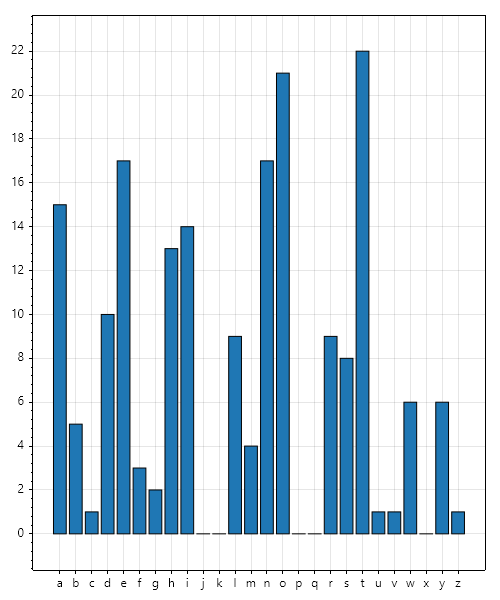
\includegraphics[width=0.7\textwidth]{original.png}
			\caption{The plaintext histogram}
			\label{fig:originalHist}
		\end{figure}
		\begin{figure}[H]
			\centering
			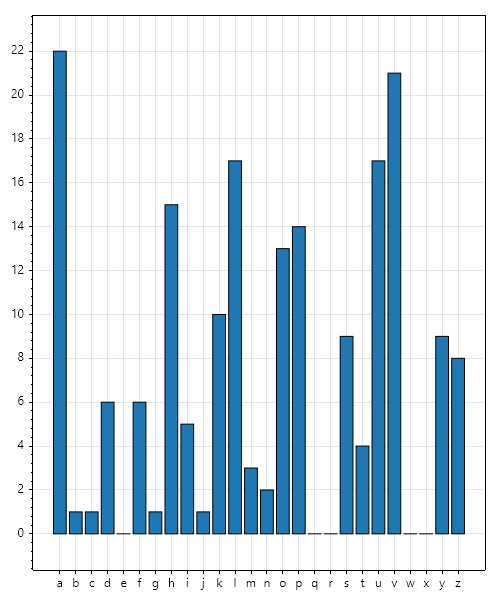
\includegraphics[width=0.7\textwidth]{shifted.png}
			\caption{Ciphertext histogram after shift cipher}
			\label{fig:shiftedHist}
		\end{figure}
		Then I generated a ciphertext using shift cipher with key $k=7$.\\
		On the histogram \ref{fig:shiftedHist} the bars' height does not change compared to the original text, only their position moves with the key. This is the key giveaway for the shift cipher.
		\begin{figure}[H]
			\centering
			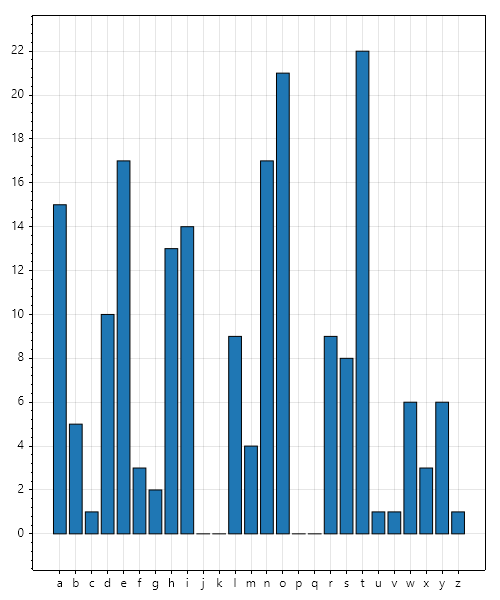
\includegraphics[width=0.7\textwidth]{permuted.png}
			\caption{Ciphertext histogram after permutation cipher}
			\label{fig:permutedHist}
		\end{figure}
		Then I generated a ciphertext with permutation cipher using the key $(7, 2, 5, 3, 8, 4, 1, 6)$, meaning the length of the key is 8. I denoted the first element with 1 in the key.\\
		The histogram \ref{fig:permutedHist} shows that all the letter frequencies remained the same, except for x, which I used to pad out the last segment of the plaintext. This is the main property for permutation ciphers, the letter frequencies do not change, only the individual letters' position.
		\begin{figure}[H]
			\centering
			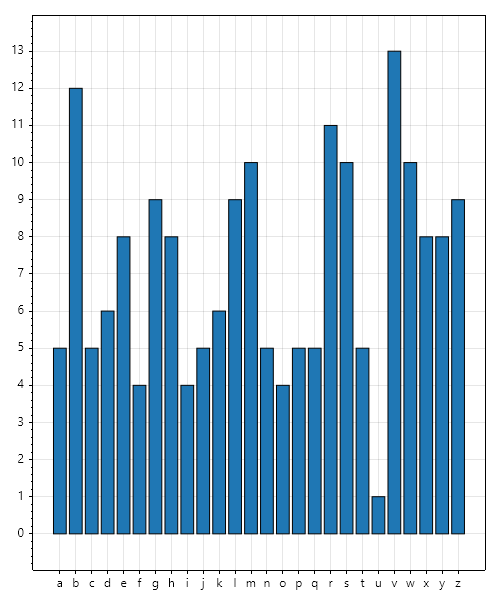
\includegraphics[width=0.7\textwidth]{vigenere.png}
			\caption{Ciphertext histogram after Vigenère cipher}
			\label{fig:vigenerelHist}
		\end{figure}
		The last ciphertext is generated with Vigenère cipher, using the key $(tolkien)$ (I felt this to be appropriate for the plaintext).\\
		The resulting histogram \ref{fig:vigenerelHist} shows a much more evenly distributed letter frequency. This is the result of each individual letter being encoded with a different individual key. The more even histogram indicates a Vigenère cipher.\\
		For each cipher I wrote the code using C\#. The histograms are generated using ScottPlot, which is a free tool for .NET. The code is available (publicly) on GitHub. \hyperlink{https://github.com/halkszavu/Encryption-Homework-2025/blob/main/Code/Homework-Calculations/Homework-Calculations/Program.cs}{Program code}
	\item \textbf{Task 3}
		
	\item \textbf{Task 4}
	\item \textbf{Task 5}
\end{enumerate}
\end{document}